\documentclass[11pt]{article}
\usepackage{placeins}
\usepackage{graphicx}
\usepackage{url}

\begin{document}

\begin{titlepage}
	\begin{center}
    	
\includegraphics[scale=0.10]{du.png}\par
		\begin{Huge}
			\textsc{University of Dhaka}\par
		\end{Huge}
		\begin{Large}
			Department of Computer Science and Engineering\par \vspace{.5cm}
			CSE-3111 : Computer Networking Lab \\[12pt]	
			Lab Report 5:Implementation of TCP flow control and congestion control algorithm (TCP Tahoe).
		\end{Large}
	\end{center}  	
	\begin{large}
		\textbf{Submitted By:\\[12pt]}
			Name : Tasfia Tabassum\\[8pt]
			Roll No : 24\\[12pt]
			Name : Saima Akter\\[8pt]
			Roll No : 30\\[12pt]
		\textbf{Submitted On : \\[12pt]}
			February 24, 2023\\[20pt]
		\textbf{Submitted To :\\[12pt]}
			Dr. Md. Abdur Razzaque\\[12pt]
                Md Mahmudur Rahman\\[12pt]
                Md. Ashraful Islam\\[12pt]
                Md. Fahim Arefin
	\end{large}
\end{titlepage}

\section{Introduction}
Transmission Control Protocol (TCP) is a widely used protocol for reliable data transmission over the internet. TCP provides end-to-end reliability by using flow control and congestion control mechanisms. Flow control is used to avoid overwhelming the receiver with too much data, while congestion control is used to prevent network congestion by adjusting the transmission rate.

TCP Tahoe is an implementation of TCP that uses a conservative approach to congestion control. It was one of the earliest TCP congestion control algorithms and is still widely used today. The main goal of TCP Tahoe is to detect congestion early and reduce the transmission rate to prevent network congestion. It achieves this by using a simple threshold-based algorithm that reduces the transmission rate by half when congestion is detected.

In this project, we will be implementing TCP Tahoe congestion control algorithm to observe its behavior in a simulated network environment. The goal of this project is to gain a deeper understanding of the TCP Tahoe algorithm and its behavior under different network conditions. 

\subsection{Objectives}
\begin{itemize}
    \item Our objective is to implement TCP Flow Control.
    
    \item Our goal is to implement TCP Congestion Control.

    \item Our aim is to analyze Analyze the captured network traffic to evaluate the performance of the TCP flow control and TCP congestion control algorithms and compare the results under different network conditions and analyze how the algorithms affect the network.
\end{itemize}
%%%%
%%%%
\section{Theory}
TCP Tahoe is a congestion control algorithm used by the Transmission Control Protocol (TCP) to regulate the transmission rate of data packets over a network. It is a simple threshold-based algorithm that aims to detect network congestion early and reduce the transmission rate to prevent network congestion from occurring.

TCP Tahoe works by maintaining a congestion window (cwnd) that determines the number of packets that can be transmitted without causing congestion. When a packet is transmitted, the cwnd is decreased by one. If an acknowledgment (ACK) is received, the cwnd is increased by one. If an ACK is not received within a timeout period, it is assumed that the packet has been lost or the network is congested, and the cwnd is reduced by half. This reduces the transmission rate, which helps to prevent network congestion.

TCP Tahoe is a conservative congestion control algorithm that reacts quickly to network congestion. However, it can result in reduced throughput if the network experiences frequent congestion. It is also vulnerable to performance degradation if there are long delays in receiving ACKs, as the timeout mechanism can result in unnecessary reductions in the transmission rate.

\section{Methodology}

\subsection{Server}
In TCP Tahoe, the server (or receiver) side operates similarly to other TCP implementations. When the server receives a packet, it sends an acknowledgment (ACK) back to the sender indicating that the packet has been received. The server also maintains a congestion window (cwnd) that determines the maximum number of packets it can receive without causing congestion.

The server uses the cwnd to control the rate at which it accepts packets. If the cwnd is smaller than the number of packets being transmitted by the sender, the server will only accept packets up to the size of the cwnd. This helps to avoid overwhelming the server with too much data and causing congestion.

If the server detects congestion, it will send a duplicate ACK to the sender, indicating that it has received a packet out of order. This is known as a fast retransmit, and it allows the sender to quickly retransmit the lost packet without waiting for a timeout. If the server receives multiple duplicate ACKs, it is an indication that there may be significant congestion on the network, and the server may reduce its cwnd to further reduce the rate of incoming packets.

Overall, the server side of TCP Tahoe operates similarly to other TCP implementations, with the main difference being the use of a threshold-based congestion control algorithm to regulate the rate of incoming packets.

\subsection{Client}
On the client side of TCP Tahoe, the sender uses a congestion control algorithm to regulate the rate of data transmission to avoid network congestion. The client maintains a congestion window (cwnd) that determines the number of packets that can be transmitted without causing congestion.

When the client sends a packet, it waits for an acknowledgment (ACK) from the server before sending the next packet. The client uses the cwnd to determine the number of packets that can be sent before waiting for an ACK. If the cwnd is smaller than the number of packets being transmitted, the client will only send packets up to the size of the cwnd. This helps to avoid overwhelming the network with too much data and causing congestion.

If the client detects congestion, it will reduce the transmission rate by reducing the size of the cwnd. In TCP Tahoe, this is done by reducing the cwnd by half when a packet is lost or when a timeout occurs. This causes the transmission rate to slow down, which helps to prevent network congestion.

TCP Tahoe also uses a slow start mechanism to gradually increase the transmission rate after congestion is detected. When congestion is detected, the cwnd is set to one, and the transmission rate is slowly increased by adding one to the cwnd for each ACK received. This allows the algorithm to slowly increase the transmission rate without causing further congestion.

Overall, the client side of TCP Tahoe operates by regulating the rate of data transmission using a congestion control algorithm that adjusts the size of the congestion window based on network conditions. This helps to ensure reliable data transmission over the network while avoiding network congestion.


\section{Implementation of TCP Flow Control}

TCP flow control is a mechanism used by the Transmission Control Protocol (TCP) to regulate the flow of data between a sender and receiver. It ensures that the receiver is not overwhelmed by too much data from the sender by controlling the rate at which data is transmitted.

TCP flow control is implemented using a sliding window protocol, where the window size represents the maximum amount of data that can be in transit at any given time. The sender continuously updates the window size based on the receiver's acknowledgments, ensuring that it does not exceed the receiver's capacity to process data.

\subsection{Algorithm to implement TCP Flow Control : }

The sender application writes data to a socket, the transport layer (in our case, TCP) will wrap this data in a segment and hand it to the network layer (e.g. IP), that will somehow route this packet to the receiving node.

On the other side of this communication, the network layer will deliver this piece of data to TCP, that will make it available to the receiver application as an exact copy of the data sent, meaning if will not deliver packets out of order, and will wait for a retransmission in case it notices a gap in the byte stream.

TCP stores the data it needs to send in the send buffer, and the data it receives in the receive buffer. When the application is ready, it will then read data from the receive buffer.

Flow Control is all about making sure we don’t send more packets when the receive buffer is already full, as the receiver wouldn’t be able to handle them and would need to drop these packets.

To control the amount of data that TCP can send, the receiver will advertise its Receive Window (rwnd), that is, the spare room in the receive buffer.

Every time TCP receives a packet, it needs to send an ack message to the sender, acknowledging it received that packet correctly, and with this ack message it sends the value of the current receive window, so the sender knows if it can keep sending data.

The sliding window : 

TCP uses a sliding window protocol to control the number of bytes in flight it can have. In other words, the number of bytes that were sent but not yet acked.

Let’s say we want to send a 150000 bytes file from node A to node B. TCP could break this file down into 100 packets, 1500 bytes each. Now let’s say that when the connection between node A and B is established, node B advertises a receive window of 45000 bytes.

Seeing that, TCP knows it can send the first 30 packets (1500 * 30 = 45000) before it receives an acknowledgment. If it gets an ack message for the first 10 packets (meaning we now have only 20 packets in flight), and the receive window present in these ack messages is still 45000, it can send the next 10 packets, bringing the number of packets in flight back to 30, that is the limit defined by the receive window. In other words, at any given point in time it can have 30 packets in flight, that were sent but not yet acked.

Now, if for some reason the application reading these packets in node B slows down, TCP will still ack the packets that were correctly received, but as these packets need to be stored in the receive buffer until the application decides to read them, the receive window will be smaller, so even if TCP receives the acknowledgment for the next 10 packets (meaning there are currently 20 packets, or 30000 bytes, in flight), but the receive window value received in this ack is now 30000 (instead of 45000), it will not send more packets, as the number of bytes in flight is already equal to the latest receive window advertised.

  \begin{figure}[!h]
\centering
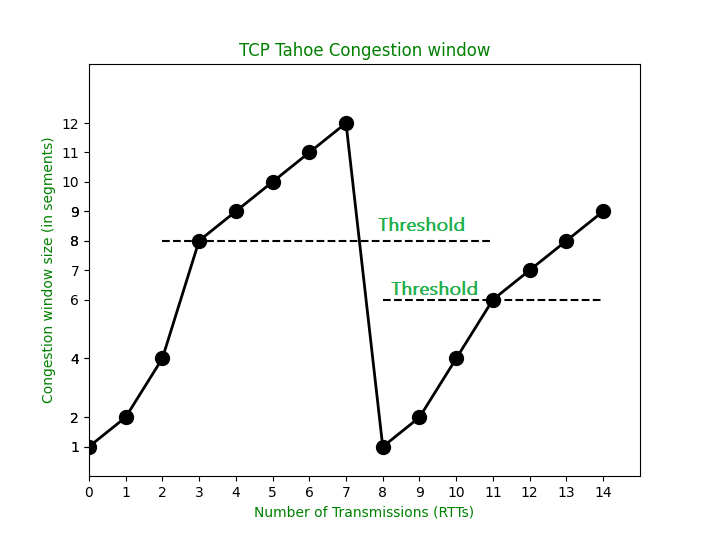
\includegraphics[width=\textwidth]{tahoecongestionwindow1.png}
\caption{ TCP Tahoe }
\end{figure}
\FloatBarrier



\subsection{Output for the Server Program}

 \begin{figure}[!h]
\centering
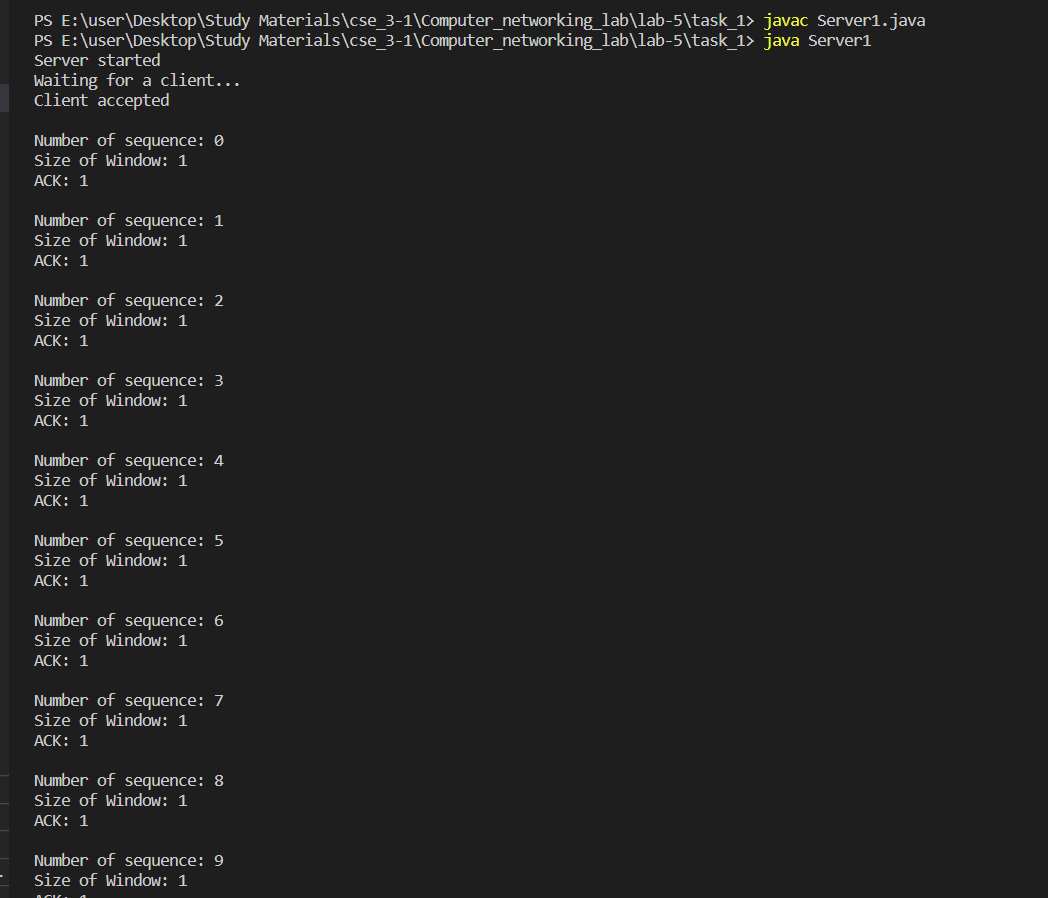
\includegraphics[width=\textwidth]{f_server1.png}
\caption{Terminal output of server java file }
\end{figure}
\FloatBarrier

\begin{figure}[!h]
\centering
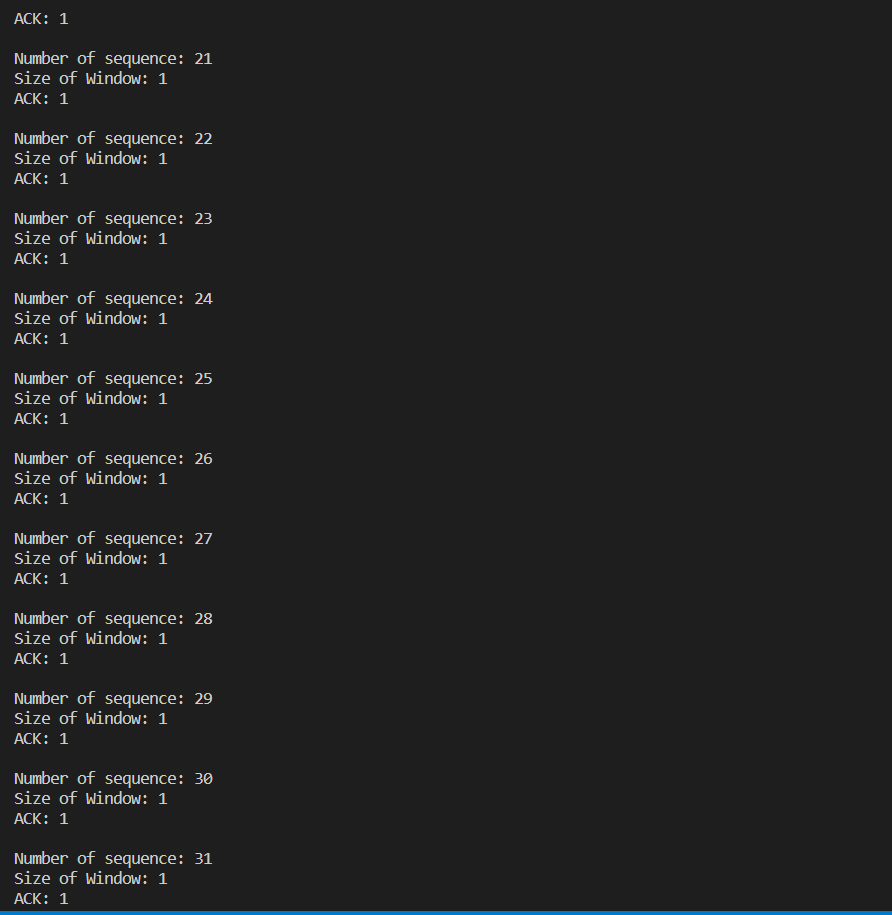
\includegraphics[width=\textwidth]{f_server2.png}
\caption{Terminal output of server java file }
\end{figure}
\FloatBarrier

\begin{figure}[!h]
\centering
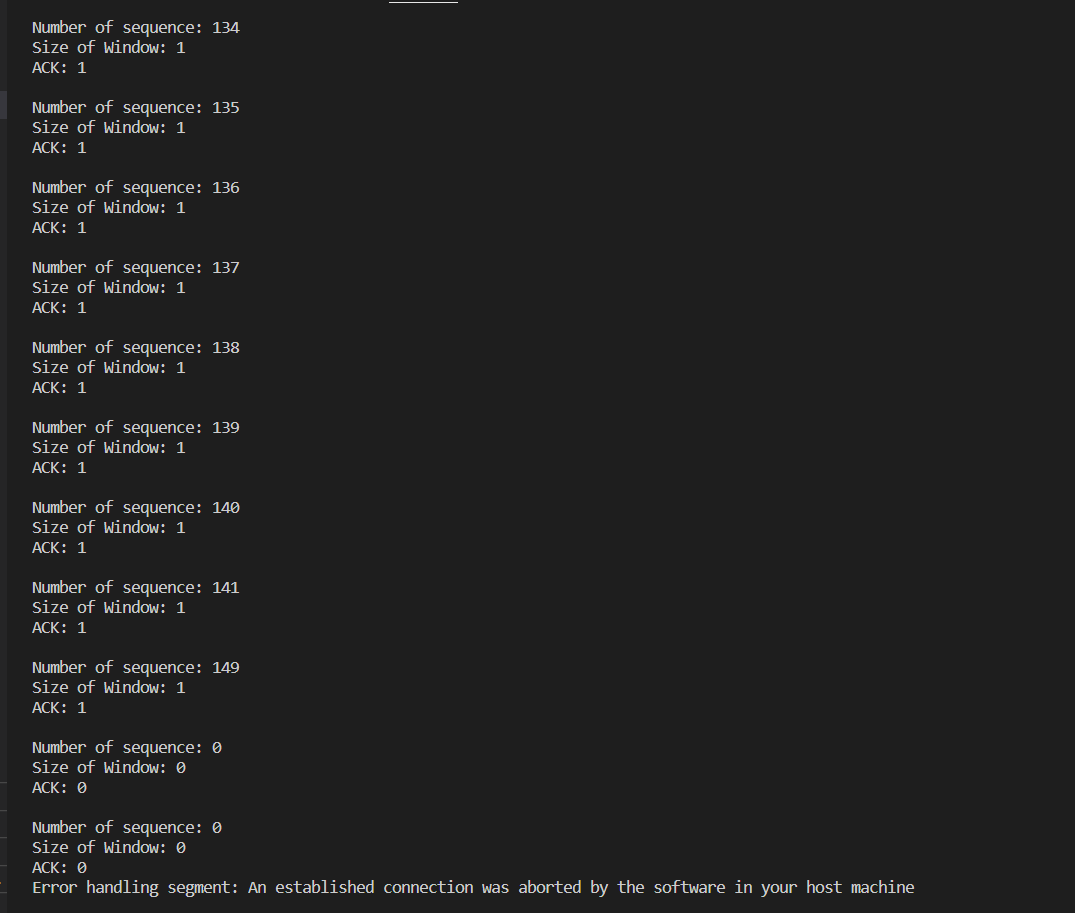
\includegraphics[width=\textwidth]{f_server3.png}
\caption{Terminal output of server java file }
\end{figure}
\FloatBarrier


\subsection{Output for the Client Program}

  \begin{figure}[!h]
\centering
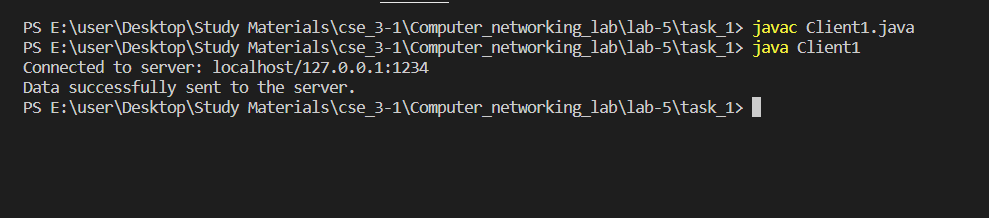
\includegraphics[width=\textwidth]{f_client.png}
\caption{Terminal output of client java file }
\end{figure}
\FloatBarrier

\section{Implementation of TCP Congestion Control}
TCP congestion control is a mechanism used by the Transmission Control Protocol (TCP) to regulate the rate of data transmission and prevent network congestion. It works by monitoring the network for signs of congestion and adjusting the rate of data transmission accordingly.

In TCP congestion control, the sender monitors the network for congestion by tracking the number of unacknowledged packets and the time it takes to receive acknowledgments. If the sender detects congestion, it reduces the rate of data transmission by reducing the size of its congestion window. This allows the network to recover from congestion and prevents further congestion from occurring.

TCP congestion control uses a variety of algorithms to regulate the rate of data transmission. One of the most commonly used algorithms is called "slow start." In slow start, the sender starts by sending a small number of packets and gradually increases the transmission rate until it detects congestion. When congestion is detected, the sender reduces the transmission rate and slowly increases it again over time.

Another common algorithm used in TCP congestion control is called "fast retransmit." In fast retransmit, the sender quickly retransmits a lost packet without waiting for a timeout, based on duplicate acknowledgments from the receiver.

Overall, TCP congestion control is an important mechanism for ensuring reliable data transmission over a network by regulating the rate of data transmission and preventing network congestion.


\subsection{Algorithm to implementation of TCP Congestion Control : }

Congestion control refers to techniques and mechanisms that can-

\begin{itemize}
    \item Either prevent congestion before it happens
    \item Or remove congestion after it has happened
\end{itemize}

TCP reacts to congestion by reducing the sender window size. The size of the sender window is determined by the following two factors-
\begin{itemize}
    \item Receiver window size
    \item Congestion window size
\end{itemize}

Receiver window size is an advertisement of how much data (in bytes) the receiver can receive without acknowledgment. Sender should not send data greater than receiver window size. Otherwise, it leads to dropping the TCP segments which causes TCP Retransmission. So, sender should always send data less than or equal to receiver window size. Receiver dictates its window size to the sender through TCP Header.
 
Sender should not send data greater than congestion window size. Otherwise, it leads to dropping the TCP segments which causes TCP Retransmission. So, sender should always send data less than or equal to congestion window size.
Different variants of TCP use different approaches to calculate the size of congestion window. Congestion window is known only to the sender and is not sent over the links.

So, 
\begin{center}
    Sender window size = Minimum (Receiver window size, Congestion window size)
\end{center}


\textbf{1. Slow Start Phase-}\\[12pt]

Initially, sender sets congestion window size = Maximum Segment Size (1 MSS). After receiving each acknowledgment, sender increases the congestion window size by 1 MSS. In this phase, the size of congestion window increases exponentially.

The followed formula is-

\begin{center}
    Congestion window size = Congestion window size + Maximum segment size
\end{center}

This phase continues until the congestion window size reaches the slow start threshold.

\begin{center}
   Threshold

= Maximum number of TCP segments that receiver window can accommodate / 2

= (Receiver window size / Maximum Segment Size) / 2
\end{center}


\textbf{2. Congestion Avoidance Phase-}\\[12pt]

After reaching the threshold, Sender increases the congestion window size linearly to avoid the congestion. On receiving each acknowledgement, sender increments the congestion window size by 1

The followed formula is-

\begin{center}
   Congestion window size = Congestion window size + 1
\end{center}

This phase continues until the congestion window size becomes equal to the receiver window size.


\textbf{3. Congestion Detection Phase-}\\[12pt]

When sender detects the loss of segments, it reacts in different ways depending on how the loss is detected-

\textbf{Case-01: Detection On Time Out-}\\[2pt]

Time Out Timer expires before receiving the acknowledgement for a segment. This case suggests the stronger possibility of congestion in the network. There are chances that a segment has been dropped in the network.

In this case, sender reacts by-

Setting the slow start threshold to half of the current congestion window size.
Decreasing the congestion window size to 1 MSS.
Resuming the slow start phase.


\textbf{Case-02: Detection On Receiving 3 Duplicate Acknowledgements-}\\[2pt]

Sender receives 3 duplicate acknowledgements for a segment. This case suggests the weaker possibility of congestion in the network. There are chances that a segment has been dropped but few segments sent later may have reached.

In this case, sender reacts by-

Setting the slow start threshold to half of the current congestion window size. Decreasing the congestion window size to slow start threshold. Resuming the congestion avoidance phase.


\subsection{Output for the Server Program}

 \begin{figure}[!h]
\centering
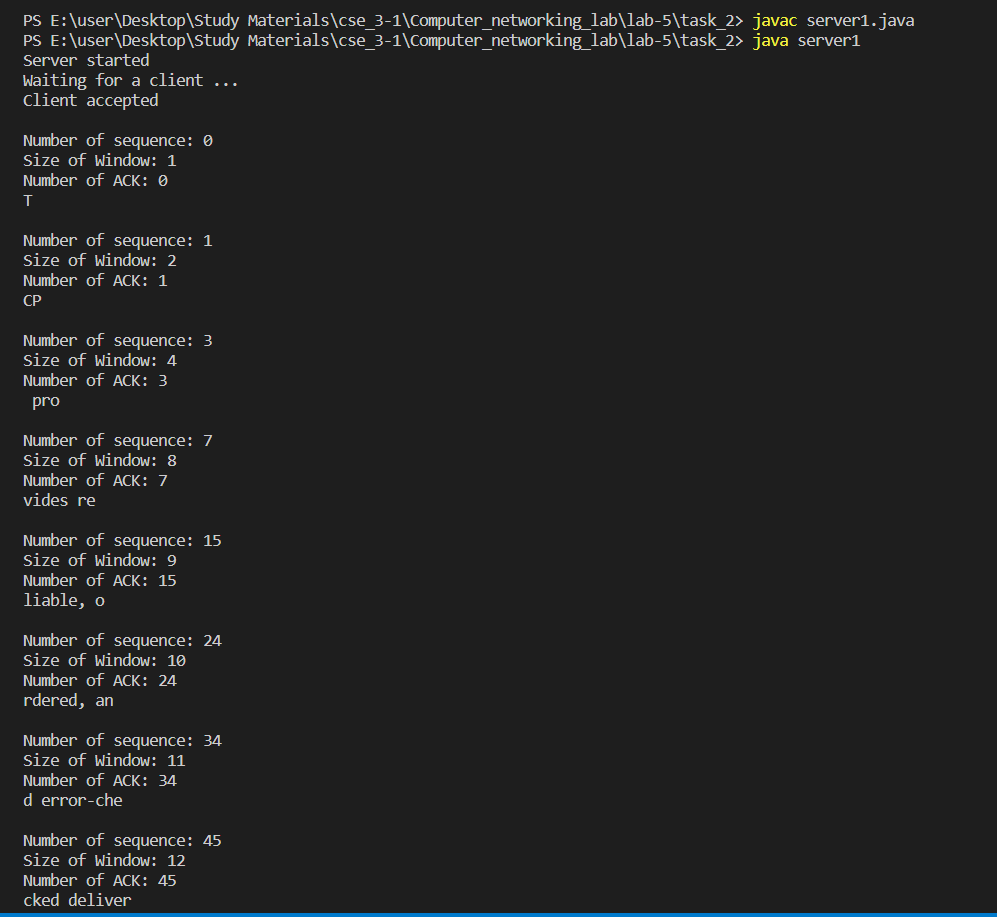
\includegraphics[width=\textwidth]{c_server1.png}
\caption{Terminal output of server java file }
\end{figure}
\FloatBarrier

\begin{figure}[!h]
\centering
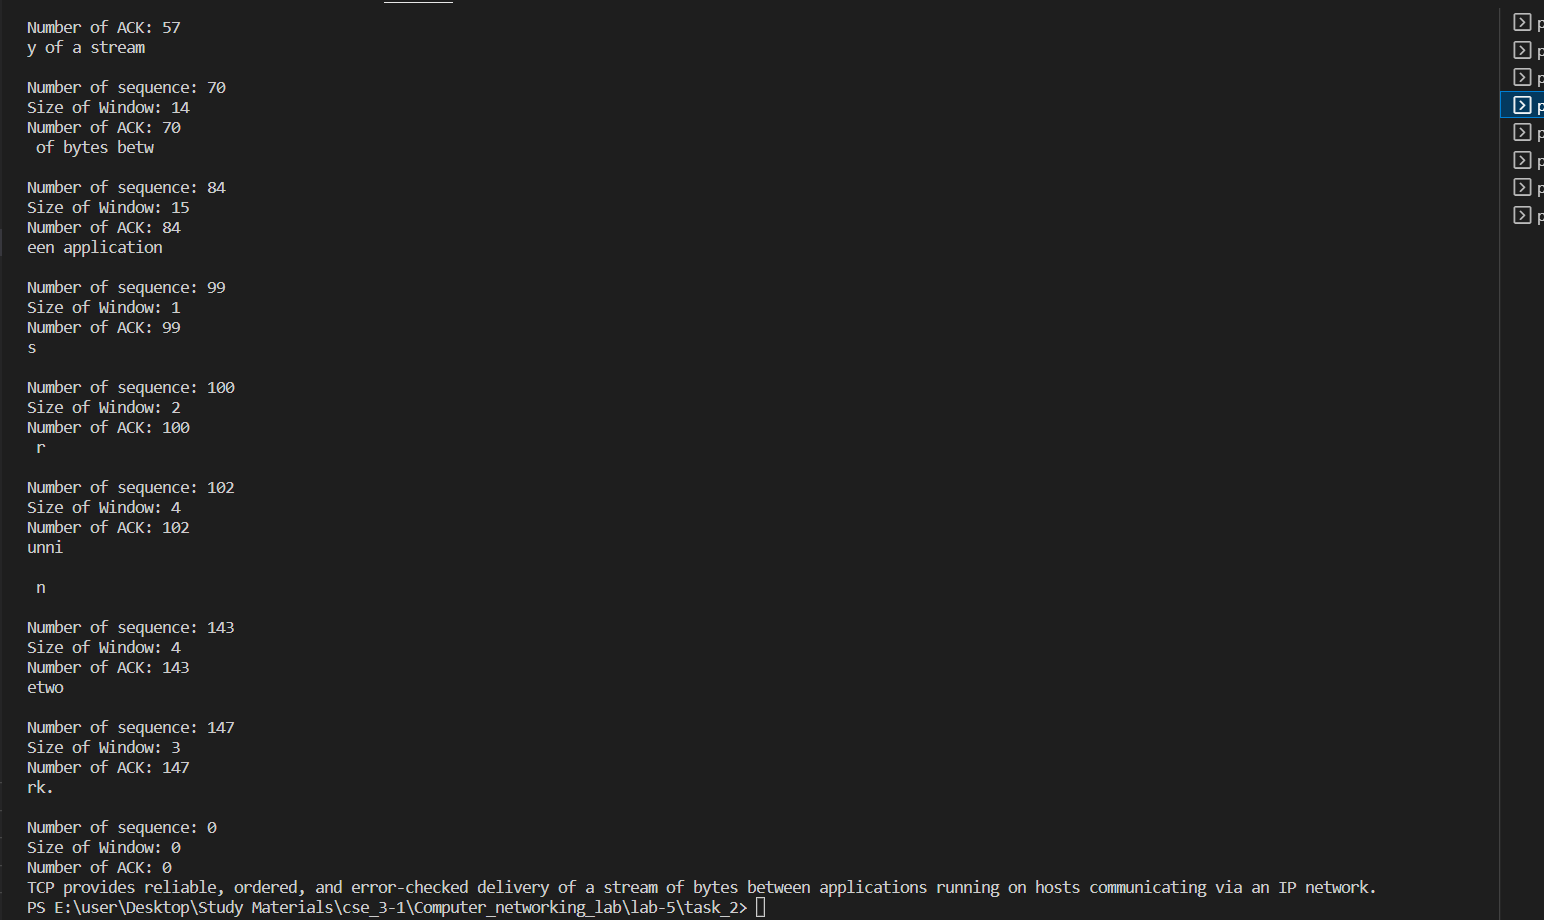
\includegraphics[width=\textwidth]{c_server2.png}
\caption{Terminal output of server java file }
\end{figure}
\FloatBarrier



\subsection{Output for the Client Program}

\begin{figure}[!h]
\centering
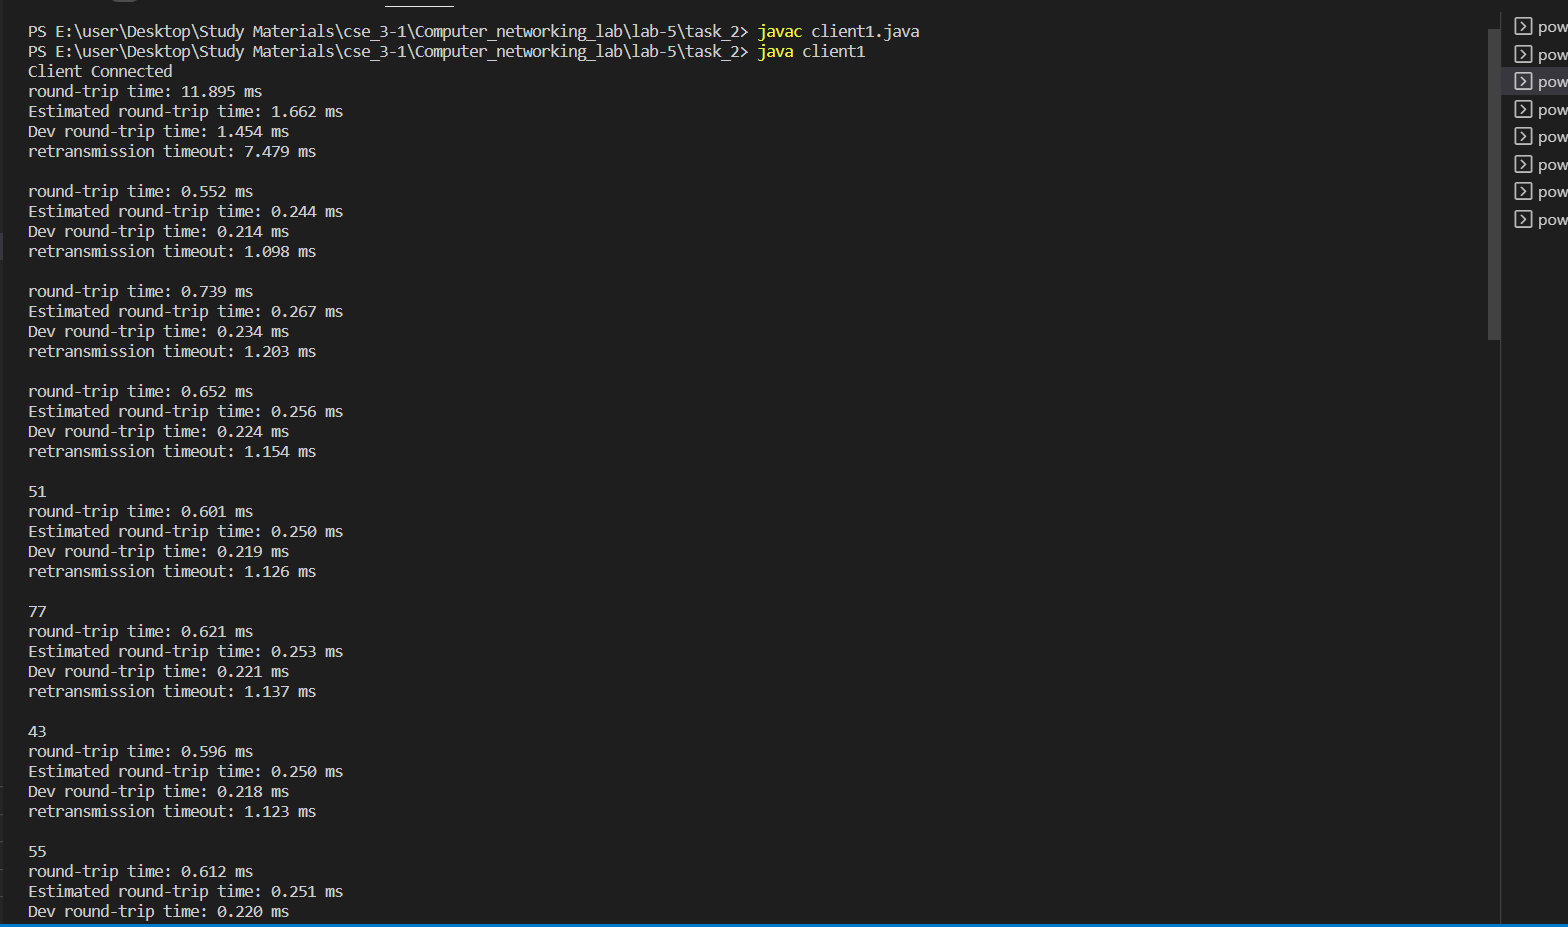
\includegraphics[width=\textwidth]{c_client1.png}
\caption{Terminal output of client java file }
\end{figure}
\FloatBarrier

  \begin{figure}[!h]
\centering
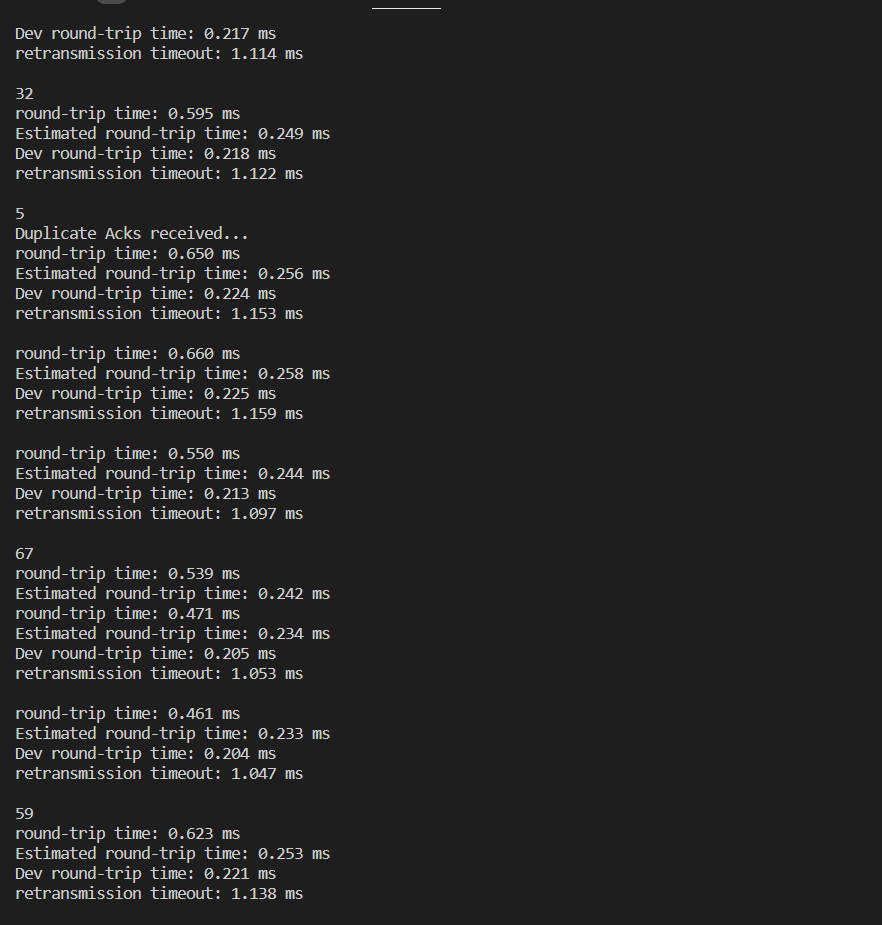
\includegraphics[width=\textwidth]{c_client2.png}
\caption{Terminal output of client java file }
\end{figure}
\FloatBarrier


\section{Analyze Results}

Analyzing captured network traffic is an essential way to evaluate the performance of TCP flow control and TCP congestion control algorithms. By examining network traffic data, we can determine how well these algorithms are working and identify any areas where they may be improved.

To evaluate TCP flow control, we can analyze the sequence of packets exchanged between the sender and receiver. Specifically, we can look at the rate of data transmission, the size of the congestion window, and the receiver's advertised window size. We can also examine the number of retransmitted packets and the round-trip time (RTT) between the sender and receiver. By comparing these metrics with expected values, we can assess the effectiveness of TCP flow control and identify any areas for improvement.

To evaluate TCP congestion control, we can examine network traffic for signs of congestion, such as packet drops, retransmissions, and increasing delays. We can also look at the size of the congestion window and how it changes over time, as well as the sender's reaction to congestion events. By comparing these metrics with expected values, we can assess the effectiveness of TCP congestion control and identify any areas for improvement.

Overall, analyzing captured network traffic is an essential tool for evaluating the performance of TCP flow control and TCP congestion control algorithms. It allows us to identify any issues or bottlenecks in the network and make improvements to ensure reliable and efficient data transmission.

\subsection{Analyze Results for  congestion control}

\subsubsection{Output for the Server Program}

 \begin{figure}[!h]
\centering
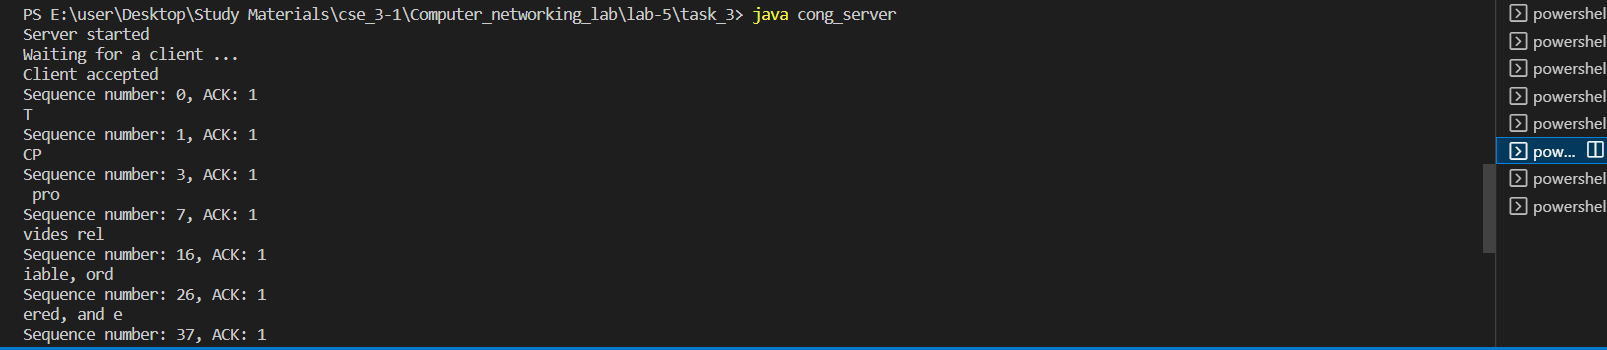
\includegraphics[width=\textwidth]{ac_server1.png}
\caption{Terminal output of server java file }
\end{figure}
\FloatBarrier

\begin{figure}[!h]
\centering
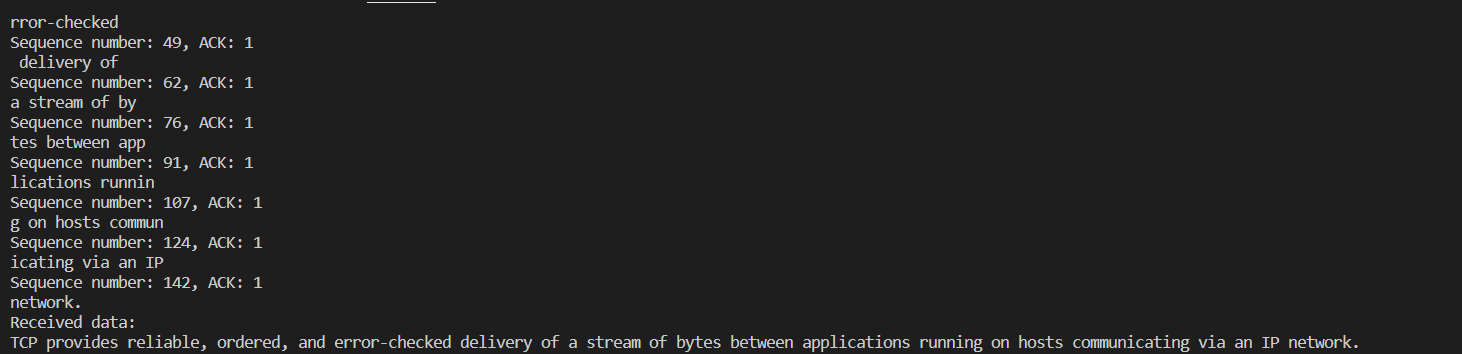
\includegraphics[width=\textwidth]{ac_server2.png}
\caption{Terminal output of server java file }
\end{figure}
\FloatBarrier



\subsubsection{Output for the Client Program}

\begin{figure}[!h]
\centering
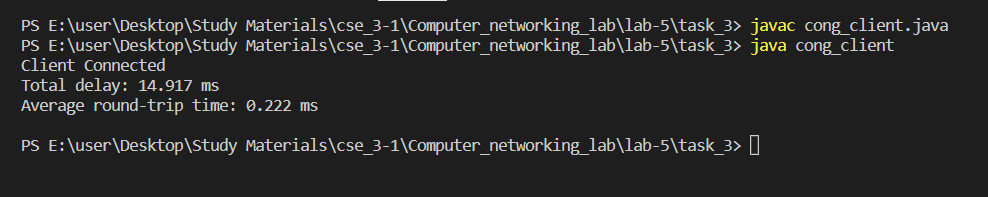
\includegraphics[width=\textwidth]{ac_client.png}
\caption{Terminal output of client java file }
\end{figure}
\FloatBarrier

 \subsection{Analyze Results for  flow control}

\subsubsection{Output for the Server Program}

 \begin{figure}[!h]
\centering
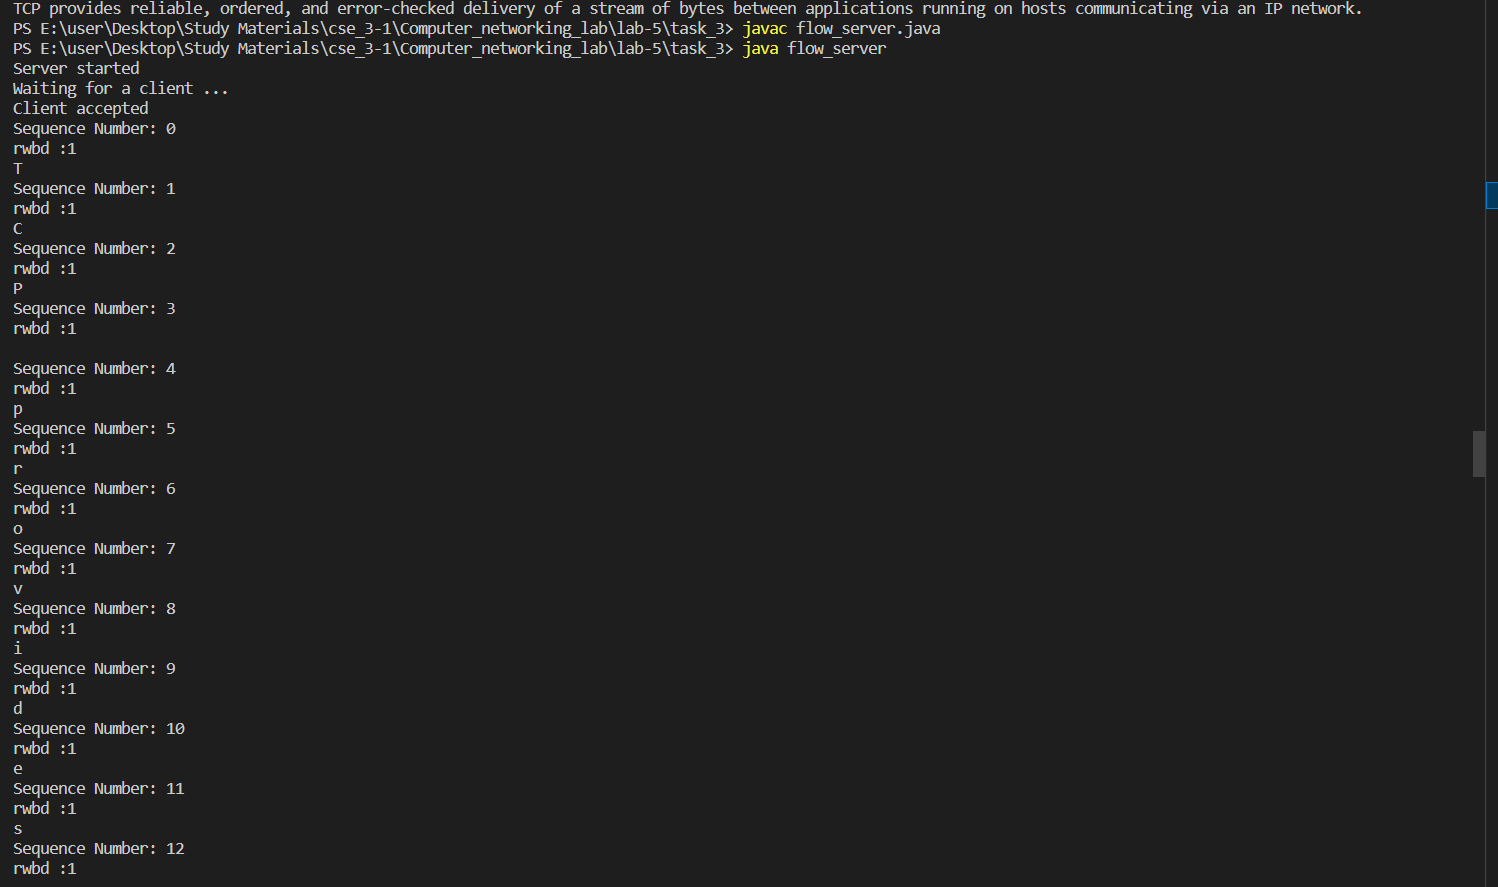
\includegraphics[width=\textwidth]{af_ser1.png}
\caption{Terminal output of server java file }
\end{figure}
\FloatBarrier

\begin{figure}[!h]
\centering
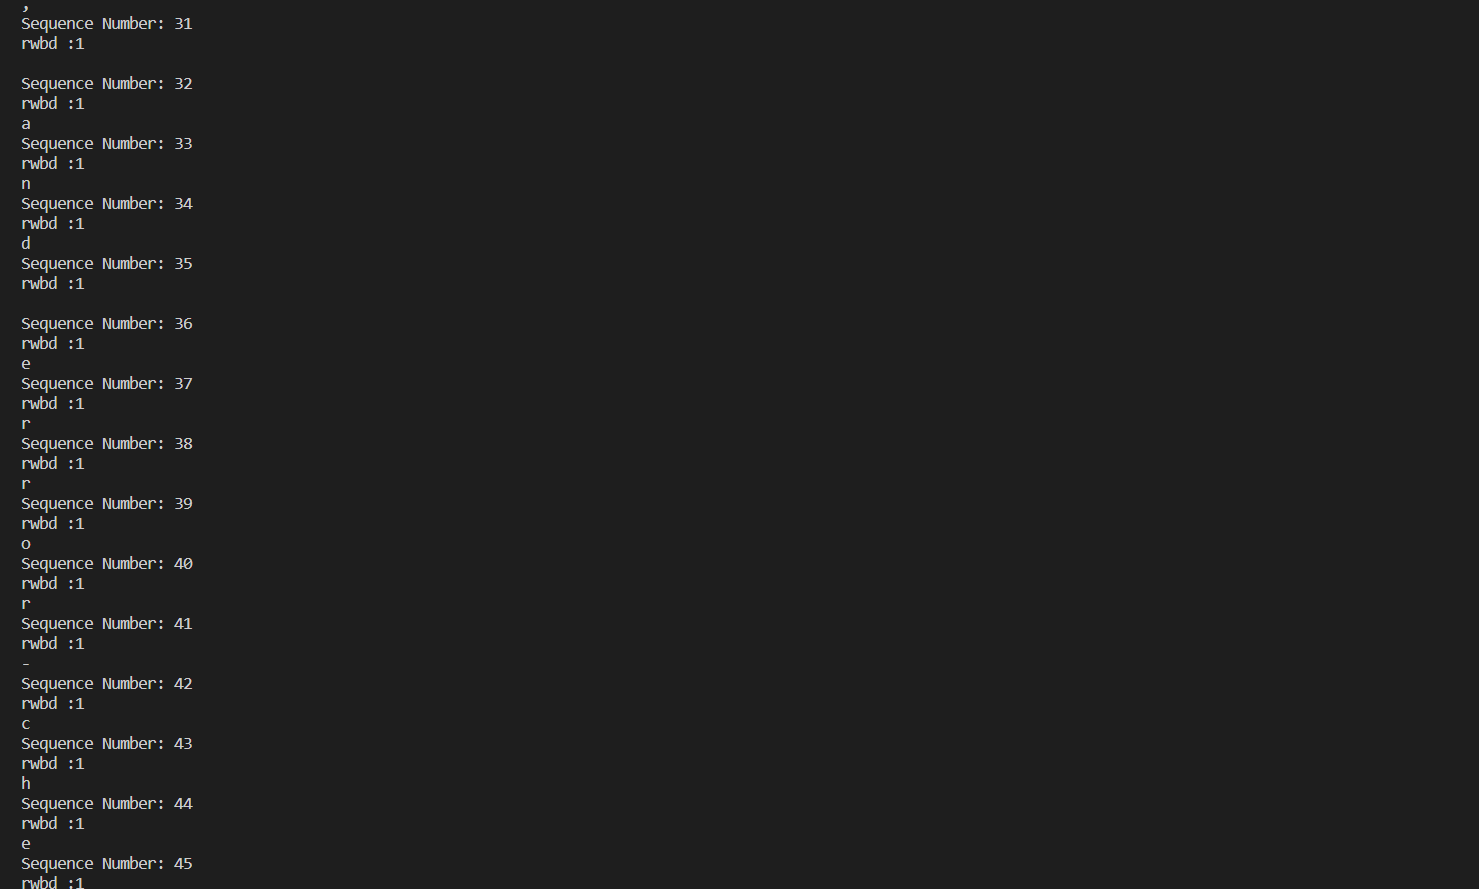
\includegraphics[width=\textwidth]{af_server2.png}
\caption{Terminal output of server java file }
\end{figure}
\FloatBarrier

\begin{figure}[!h]
\centering
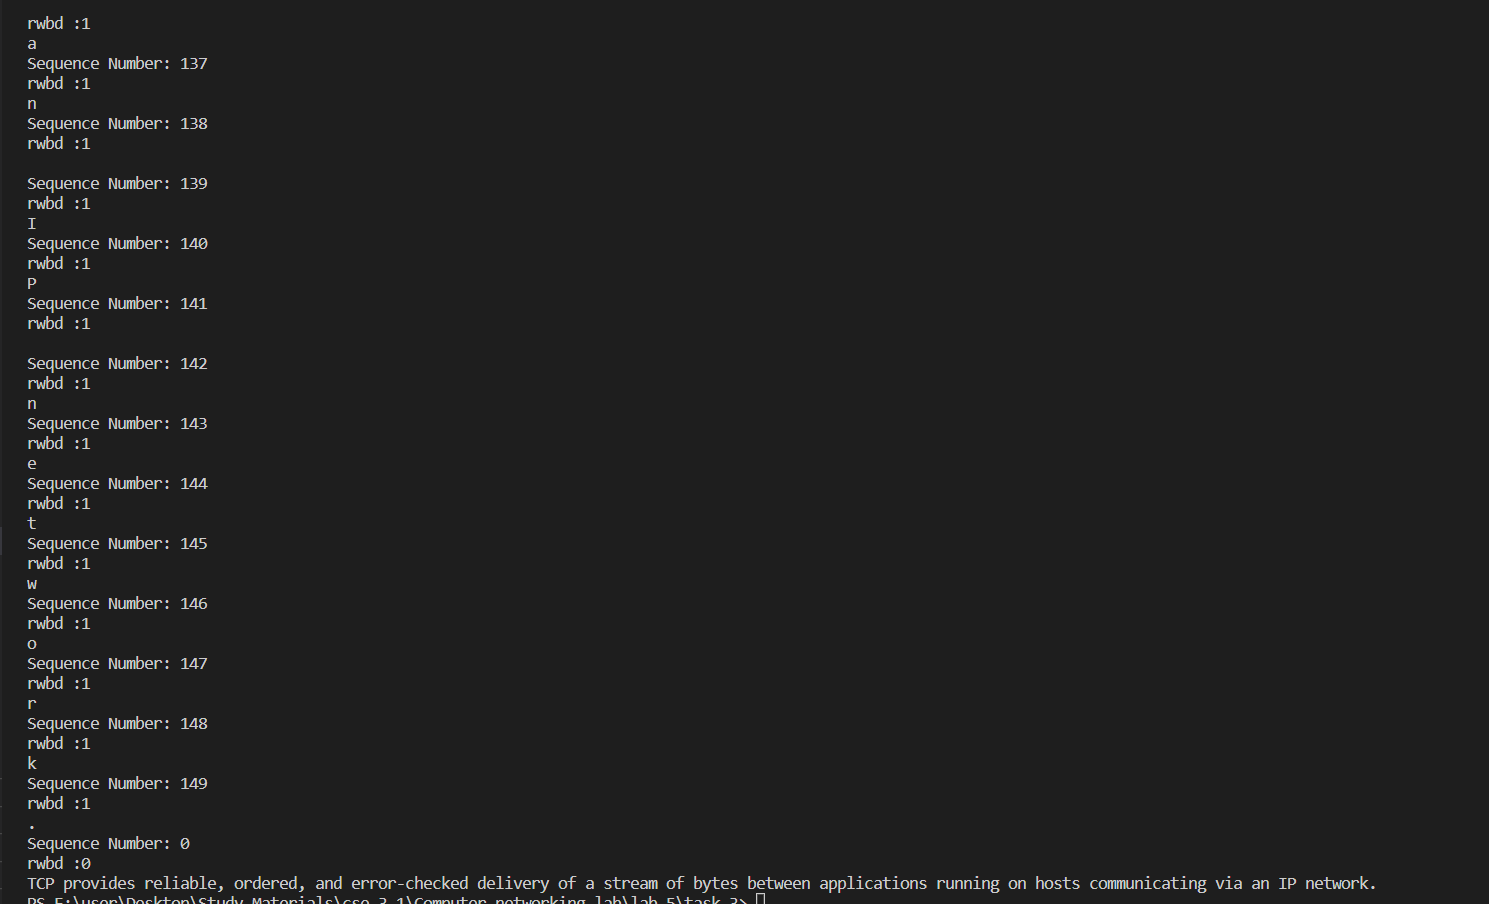
\includegraphics[width=\textwidth]{af_server3.png}
\caption{Terminal output of server java file }
\end{figure}
\FloatBarrier

\subsubsection{Output for the Client Program}

\begin{figure}[!h]
\centering
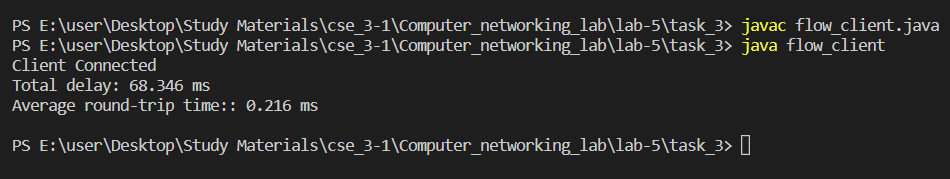
\includegraphics[width=\textwidth]{af_client.png}
\caption{Terminal output of client java file }
\end{figure}
\FloatBarrier


\section{Experience}
In the lab report on "Implementation of TCP flow control and congestion control algorithm (TCP Tahoe)" we conducted a comprehensive study on an implementation of TCP that uses a conservative approach to congestion control and flow control. Through this, we got a better understanding of how not to overwhelm the receiver with more data than it can handle and how to prevent congestion in the network. 



\begin{thebibliography}{1}
\bibitem{book}  Computer networking : a top-down approach 6th ed.
\bibitem{StackOverflow} StackOverflow : \url{http://stackoverflow.com/}
\bibitem{Geeks for geeks} GeeksforGeeks : \url{https://www.geeksforgeeks.org/}
\end{thebibliography}

\end{document}